%\vspace{1.5pc}
\vspace{1.5pc}
%\section[State of the Art]{State of the Art}
\begin{spacing}{1.5}
	
	Bab ini menjelaskan lebih detail mengenai pustaka relevan dan tinjauan teori dalam penelitian ini. Hal ini bertujuan untuk mereview, mengupdate, mengkritik dan mensintesis literatur, melakukan meta-analisis literatur, melakukan konsepsi ulang dari topik yang direview, dan menjawab pertanyaan spesifik penelitian dari topik yang telah direview dalam literatur \shortcite{Torraco2016}. Struktur pembahasan studi relevan dan tinjauan teori selanjutnya dibagi dalam beberapa hal: pertama, akan dibahas mengenai persamaan gerak fluida dan persamaan Navier-Stokes dalam pemodelan laut, serta grid C Arakawa. Selanjutnya, akan dibahas mengenai model iklim yang digunakan dan terakhir tentang kedalaman lapisan campuran. Meskipun demikian, karena fokus dari penelitian ini adalah observasi kedalaman lapisan campuran berdasarkan data output OGCM (\textit{Ocean General Circulation Model}) dan hubungan serta pengaruh parameter meteorologi terhadap lapisan campuran, maka persamaan Navier-Stokes tidak akan direview secara detail dan hanya akan dirujuk sebagaimana mestinya.
	
\end{spacing}
\vspace{-0.1pc}
\section[Persamaan Gerak Fluida]{Persamaan Gerak Fluida}
\begin{spacing}{1.5}
	
	Persamaan matematika yang mengatur aliran viskoelastik fluida berasal dari persamaan-persamaan hukum konservasi fisika yaitu konservasi massa, momentum dan persamaan konstitutif reologi \shortcite{Alves2021}. Penjabaran dari hukum-hukum tersebut menentukan bagaimana suatu persamaan model hidrodinamika dibuat. Salah satu persamaan fluida yang paling terkenal adalah persamaan Navier-Stokes yang terdiri dari persamaan momentum, persamaan kontinuitas, dan persamaan konservasi densitas \shortcite{Haditiar2020}. Persamaan Navier-Stokes digunakan untuk menggambarkan fluida yang mengalir dan dianggap memiliki pergerakan yang kontinu. Diketahui bahwa hasil pengamatan dari sebuah partikel fluida yang mengalir memiliki sifat-sifat fluida secara umum yaitu kecepatan, temperatur, tekanan dan densitas \shortcite{Rafiq2019,Das2018,Khan2019}. Sebuah partikel fluida diilustrasikan pada Gambar \ref{fig:cube}a, dan \ref{fig:cube}b. Komponen fluida seperti tekanan ($p$), kecepatan ($u$), dan densitas ($\rho$) terletak pada pusat partikel yang bergantung terhadap waktu $(t)$ dan ruang $(x,y,z)$, sehingga komponen-komponen tersebut dapat ditulis dalam bentuk fungsi tekanan $p(x,y,z,t)$, fungsi kecepatan $u(x,y,z,t)$  dan fungsi densitas $\rho(x,y,z,t)$. 
	
	Misalkan ke-enam sisi kubus sebagai $N, S, E, W, I$, dan $B$ seperti yang ditunjukkan dalam Gambar \ref{fig:cube}a. Selanjutnya asumsikan bahwa partikel fluida yang diobservasi sangat kecil sehingga sifat fluida pada permukaan kubus dapat diekspresikan secara akurat dengan menggunakan rata-rata dua suku pertama dari ekspansi deret Taylor, 
	\begin{equation*}
		\sum_{n=0}^{\infty}\frac{f^{n}(a)}{n!}(x-a)^n = f(a)+\frac{f'(a)}{1!}(x-a)+\dots.
	\end{equation*}
 
	Perhatikan bahwa $f$ di atas dapat berupa $p(x,y,z,t), u(x,y,z,t)$ atau $\rho(x,y,z,t)$. Sebagai contoh, densitas pada sisi kubus $W$ dan $E$. Keduanya memiliki jarak $\frac{1}{2}\delta x$ dari posisi partikel yang berada di tengah, sehingga diperoleh bentuk ekspresi
	\begin{equation*}
		\rho-\frac{\partial \rho}{\partial x}\frac{1}{2}\delta x \quad \text{dan} \quad
		\rho+\frac{\partial \rho}{\partial x}\frac{1}{2}\delta x.
	\end{equation*}
	Dalam hal ini, $\rho$ adalah densitas, $\frac{\partial \rho}{\partial x}$ adalah laju perubahan densitas terhadap posisi $x$, dan $\delta x$ adalah panjang rusuk kubus.
	\begin{figure}[H]
		\centering
		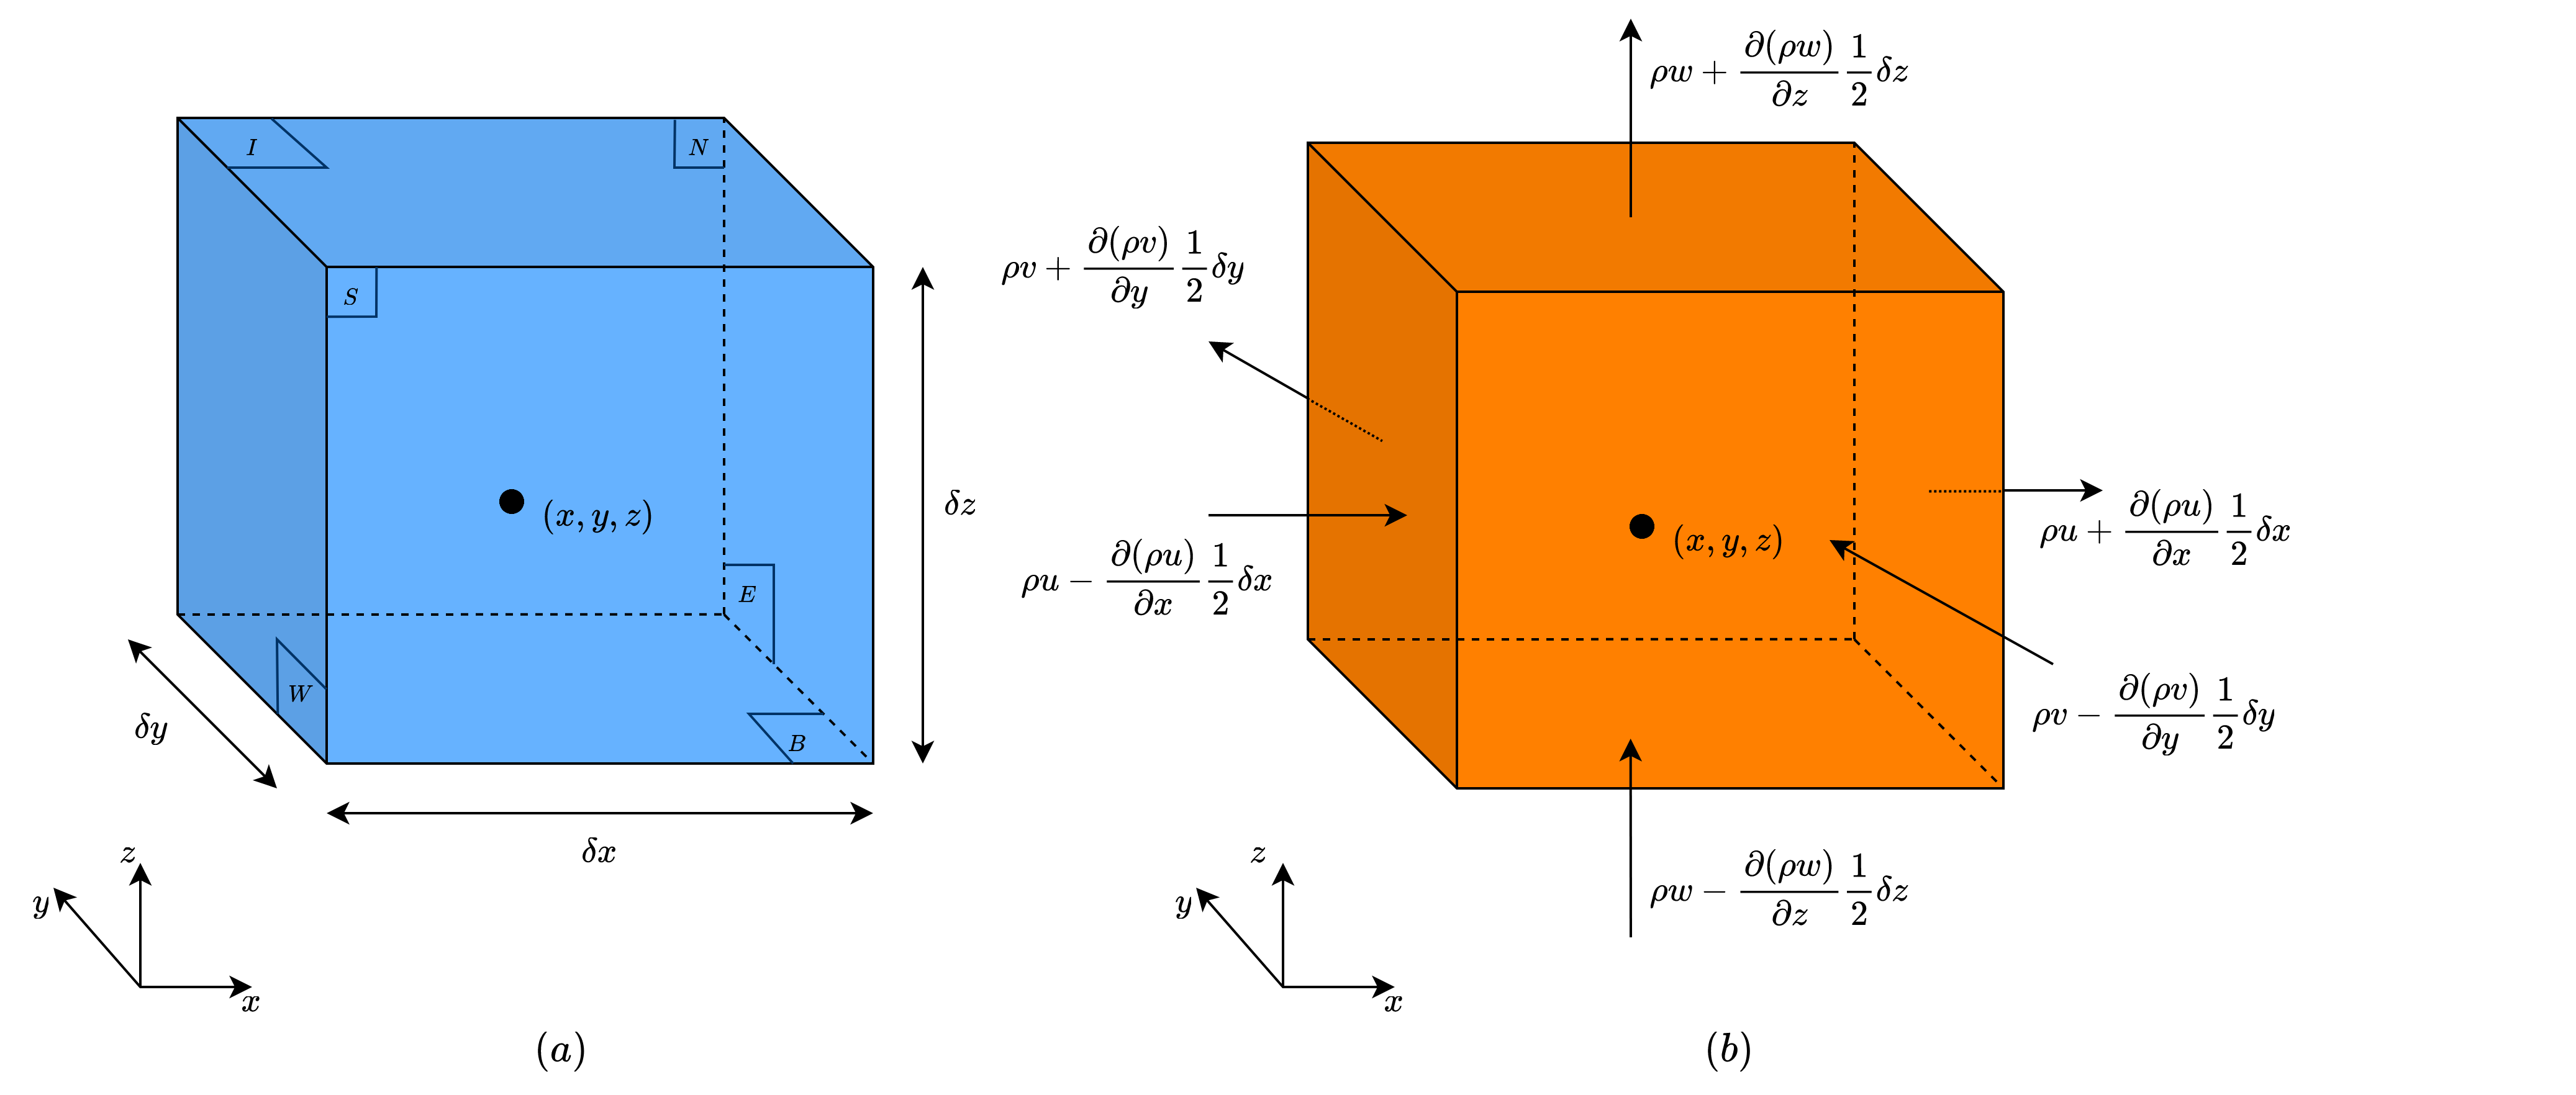
\includegraphics[width=16cm]{contents/cube}
		\caption{(a) Ilustrasi partikel sebagai sifat fisis fluida, (b) Aliran massa jenis masuk dan keluar. Gambar direproduksi dari \protect\shortcite{versteeg2007introduction}.}
		\label{fig:cube}
	\end{figure}
	Densitas atau massa jenis dari partikel $\rho(x,y,z,t)$ pada Gambar \ref{fig:cube}(a) dapat diterjemahkan sebagai aliran yang masuk dan keluar. Pada Gambar \ref{fig:cube}(b), arah aliran massa jenis pada partikel pusat merupakan jumlahan dari aliran massa jenis masuk dan keluar. Dengan cara yang sama dapat juga dilakukan untuk tekanan dan kecepatan. 
\end{spacing}
\vspace{-1pc}
\section[Persamaan Primitif]{Persamaan Primitif}
\begin{spacing}{1.5}
	\par Model sirkulasi laut atau \textit{Ocean General Circulation Models} (OGCM) menggunakan persamaan Navier-Stokes untuk memodelkan fenomena fisis yang terjadi di lautan. Lautan adalah fluida yang dapat dijelaskan dengan baik dengan pendekatan persamaan-persamaan primitif, yaitu persamaan Navier-Stokes bersama dengan persamaan keadaan nonlinier yang menggabungkan dua variabel (temperatur dan salinitas) dengan kecepatan fluida, ditambah dengan pertimbangan beberapa asumsi dan hipotesis \shortcite{madec_gurvan_2022_6334656}.
	
	Beberapa hipotesis yang digunakan dalam persamaan Navier-Stokes adalah hipotesis Boussinesq, hipotesis hidrostatik, dan hipotesis tak termampatkan (\textit{incompressibility}). Berdasarkan hipotesis Boussinesq, variasi densitas diabaikan kecuali dalam kontribusinya terhadap gaya apung sehingga 
	\begin{equation}\label{eq:P1}
		\rho = \rho(T,S,p)
	\end{equation}
	dengan $\rho$ adalah densitas in situ, $T$ adalah potensial temperature, $S$ adalah salinitas, dan $p$ adalah tekanan.
	Untuk hipotesis hidrostatik, persamaan momentum vertikal direduksi menjadi keseimbangan antara gradien tekanan vertikal dan gaya apung
	\begin{equation}
		\frac{\partial p}{\partial z} = -\rho g.
	\end{equation}
	Untuk hipotesis tak termampatkan, persamaan 3-D divergensi untuk vektor kecepatan $U = (u,v,w)$ (dalam koordinat kartesius $(x,y,z)$) diasumsikan menjadi 0, diperoleh
	\begin{equation}
		\nabla \;.\; U =\frac{\partial u}{\partial x} + \frac{\partial v}{\partial y} + \frac{\partial w}{\partial z} = 0.
	\end{equation}	

	Selanjutnya misalkan bahwa $U$ adalah vektor kecepatan dengan $U = U_h + wk$ ($h$ adalah notasi vektor horizontal lokal di atas bidang $(i,j)$), $T$ adalah temperatur potensial, $S$ adalah salinitas, $\rho$ adalah densitas in situ. Bentuk vektor invarian dari persamaan primitif dalam sistem vektor $(i, j, k)$ diberikan oleh persamaan berikut \shortcite{madec_gurvan_2022_6334656},
	
	- Persamaan kesetimbangan momentum
	\begin{equation}\label{eq:P2}
		\begin{aligned}
			\frac{\partial U_h}{\partial t} = - \left[(\nabla \times U) \times U + \frac{1}{2}\nabla (U^2)\right]_h - f \; k \times U_h - \frac{1}{\rho_o}\nabla_h p + D^U + F^U.
		\end{aligned}
	\end{equation}

	- Persamaan konservasi panas dan salinitas
	\begin{equation}\label{eq:P3}
		\begin{aligned}
			\frac{\partial T}{\partial t} &= - \nabla \; . \; (T\;U)  + D^U + F^U \\
			\frac{\partial S}{\partial t} &= - \nabla \; . \; (S\;U)  + D^U + F^U.
		\end{aligned}
	\end{equation}
	Dengan $\nabla$ operator vektor turunan yang diperumum dalam arah $(i,j,k)$, $t$ adalah waktu, $z$ adalah koordinat vertikal, $\rho$ adalah densitas in situ dalam persamaan keadaan hipotesis Boussinesq, $\rho_o$ adalah densitas referensi, $p$ adalah tekanan, $f = 2\Omega\; . \;k$ adalah percepatan Coriolis (dengan $\Omega$ adalah vector kecepatan sudut bumi), $g$ adalah percepatan gravitasi. $D^U, D^T$, dan $D^S$ adalah parameterisasi dari fisika skala kecil  untuk momentum, temperatur, dan salinitas, dan $F^U,F^T$, dan $F^S$ adalah suku gaya permukaan.
	 
	Dalam aplikasinya, persamaan Navier-Stokes tidak hanya digunakan untuk memodelkan laut, tapi juga merambah ke bidang pemodelan cuaca \shortcite{Rohli2021}, aliran air dalam pipa \shortcite{Ouchiha2012} dan aliran udara di sekitar sayap pesawat \shortcite{Tulus2019}. Dalam bentuk persamaan lengkap dan simplifikasi, persamaan ini juga dapat digunakan untuk mendesain kereta api \shortcite{Croquer2020}, pesawat terbang \shortcite{Chau2021}, dan mobil \shortcite{Ambarita2018}. Terdapat juga studi tentang aliran darah \shortcite{Gill2021}, desain stasiun pembangkit listrik \shortcite{Yang2019}, dan analisis polusi udara \shortcite{Issakhov2022}. 

\section[Arakawa C grid]{Arakawa C grid}
	Diskritisasi grid di bidang horizontal dapat dibedakan menjadi grid persegi (\textit{rectiliniear}) Gambar \ref{fig:grid}a dan grid lengkung (\textit{curvlinear}) Gambar \ref{fig:grid}b, di bidang vertikal berupa grid level z (\textit{z-coordinates}) Gambar \ref{fig:grid}c dan grid level s (\textit{$\sigma$-coordinate}) Gambar \ref{fig:grid}d \shortcite{Delandmeter2019}.
	
	\begin{figure}[H]
		\centering
		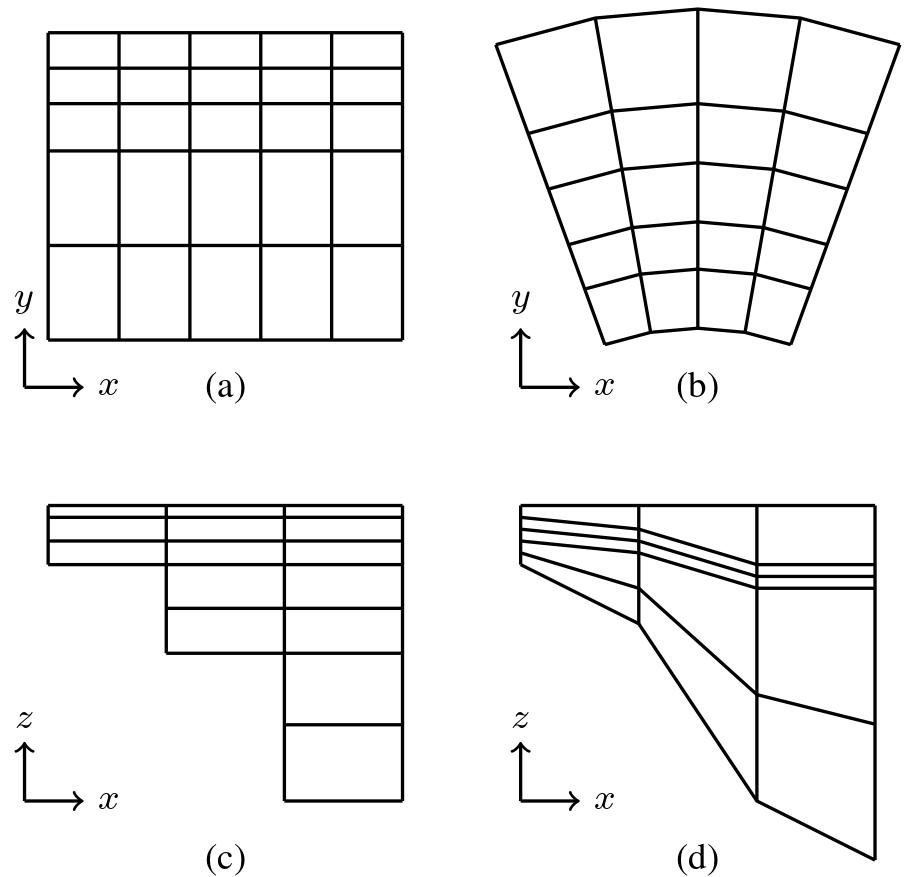
\includegraphics[width=7cm]{contents/grid.jpg}
		\caption{Jenis grid dalam pemodelan laut. Di bidang horizontal: (a) grid persegi, (b) grid lengkung, di bidang vertikal: (c) grid level z, (d) grid level s \protect\shortcite{Delandmeter2019}.}
		\label{fig:grid}
	\end{figure}
	
	Dalam aplikasinya, beberapa software pemodelan laut mengimplementasikan grid bertingkat (\textit{staggered grid}) yang diperkenalkan oleh \shortciteNP{ARAKAWA1977}, yaitu grid A, B dan C. Lebih lanjut, antara grid A, dan grid C terdapat perbedaan fundamental yaitu letak penyimpanan simpul variabel (lihat Gambar \ref{fig:arakawa}), sedangkan grid B dapat dianggap sebagai peralihan dari grid A ke grid C dan perbedaan tipe model grid ini menjadi penting dikarenakan peningkatan kapasitas komputasi yang stabil di banyak pusat pemodelan iklim telah mengantarkan periode transisi untuk model laut global  \shortcite{Barham2018,Delandmeter2019}. 
	
	\begin{figure}[H]
		\centering
		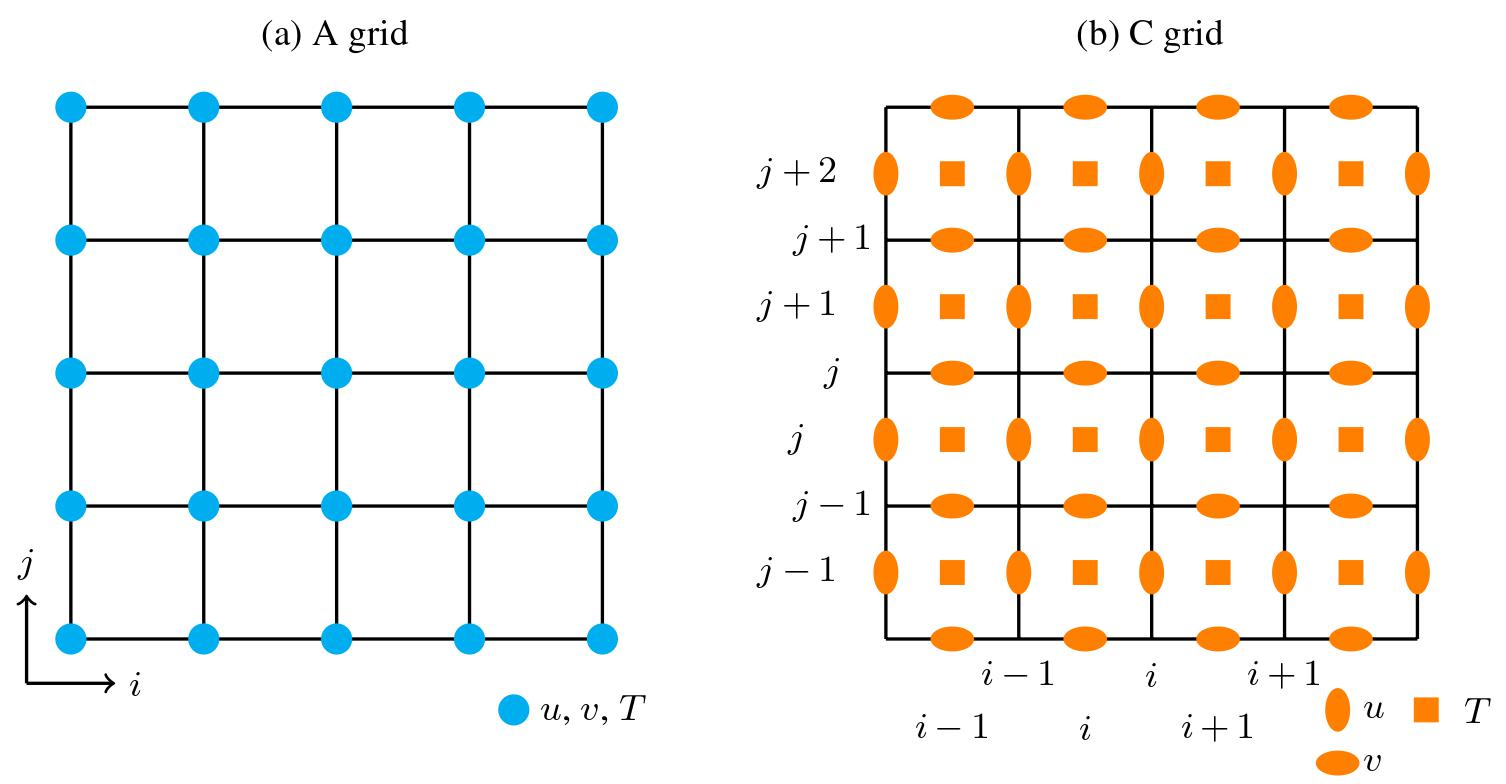
\includegraphics[width=13cm]{contents/arakawa.jpg}
		\caption{Grid Arakawa: (a) Grid A dan (b) Grid C \protect\shortcite{Delandmeter2019}}
		\label{fig:arakawa}
		\medspace
		\small
		Grid A adalah satu-satunya \textit{unstaggered grid} dalam grid Arakawa dimana variabel-variabelnya (\textit{zonal velocity (u), meridional velocity (v), tracers (T)}) hanya terdapat pada titik sudut grid, berbeda dengan grid C yang berada di sisi dan tengah grid. $i$ dan $j$ adalah indeks yang merepresentasikan variabel kolom dan baris dimana variabel disimpan.
	\end{figure}
\end{spacing}
\vspace{-0.1pc}
\section[Sistem Koordinat]{Sistem Koordinat}
\begin{spacing}{1.5}
	Dalam arah horizontal, model menggunakan grid ortogonal lengkung sedangkan dalam arah vertikal, model menggunakan langkah \textit{full} atau sebagian untuk koordinat z, atau koordinat s, atau campuran keduanya. Distribusi variabel adalah grid tipe Arakawa C tiga dimensi.
\subsection[Sistem Koordinat-z Lengkung]{Sistem Koordinat-z Lengkung}
	Mengingat sistem koordinat geografis demikian kompleks, maka penting untuk menyelesaikan persamaan primitif dalam berbagai sistem koordinat lengkung. Cara terbaik untuk menunjukkan transformasi koordinat adalah formalisme tensorial. Persamaan sederhana untuk kasus grid ortogonal 3-D pada bidang (perkiraan bumi bulat) dapat diilustrasikan sebagai berikut.
	\begin{figure}[H]
		\centering
		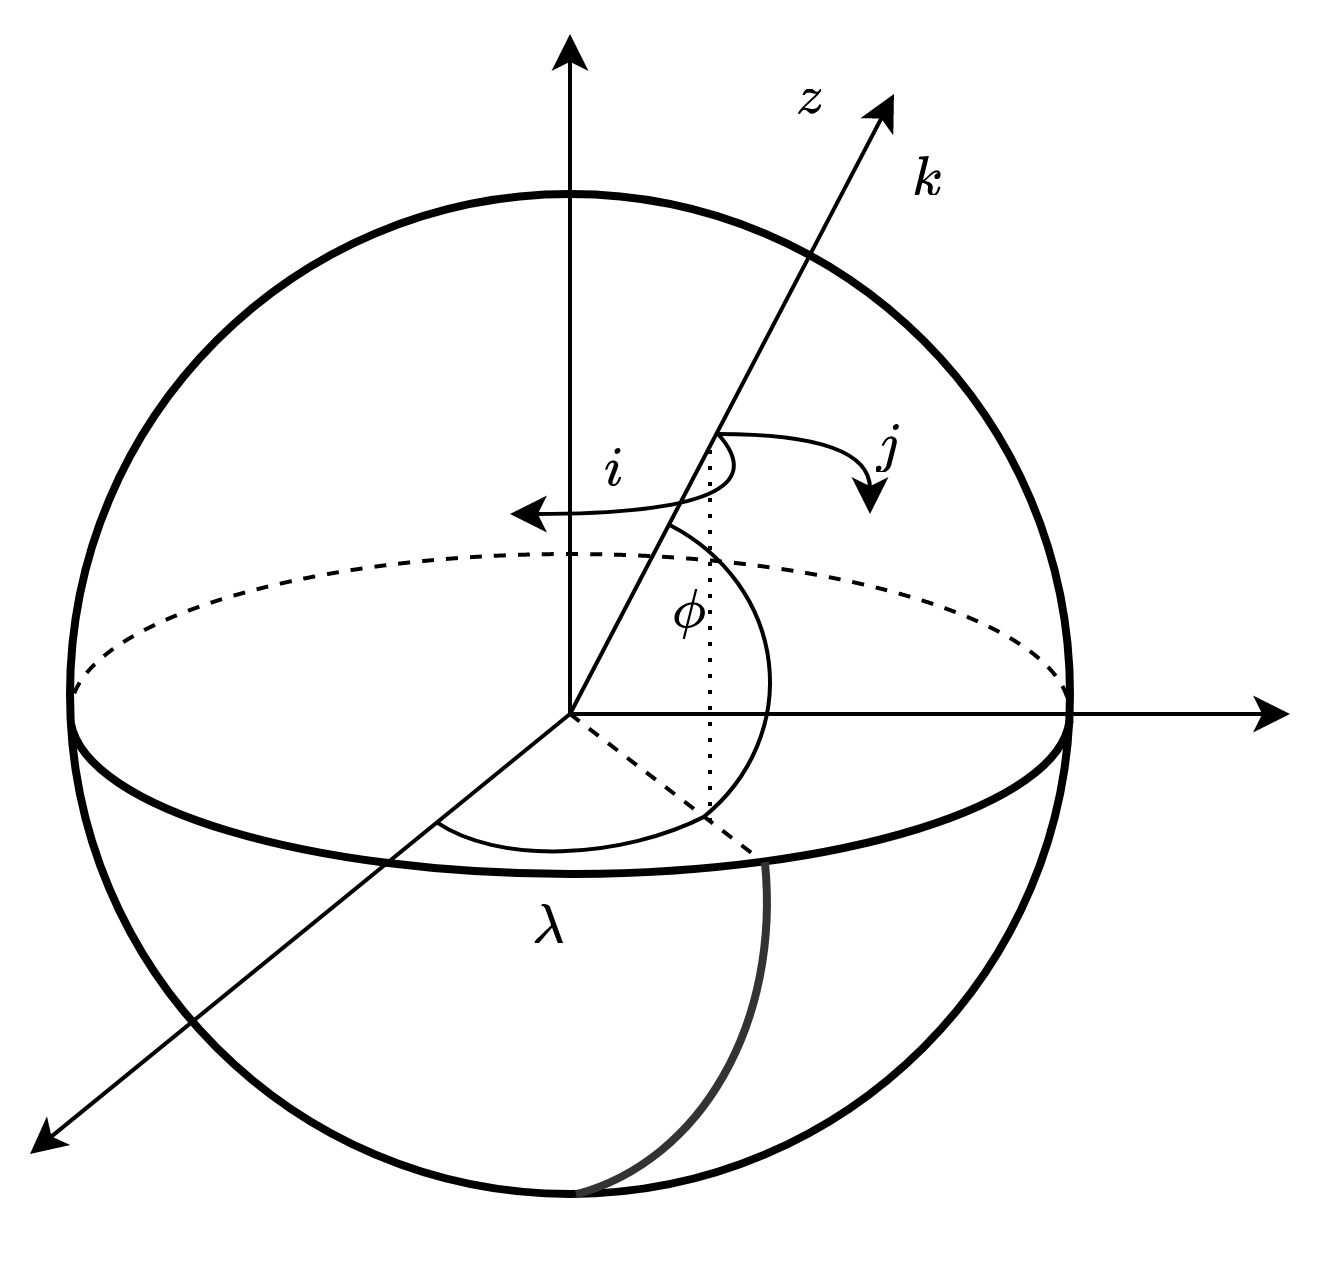
\includegraphics[width=7cm]{contents/sphere.png}
		\caption{Sistem koordinat geografis ($\lambda, \phi,z$) dan sistem koordinat lengkung ($i,j,k$) \protect\shortcite{madec_gurvan_2022_6334656}}.
		\label{fig:sphere}
	\end{figure}
	Misal ($i,j,k$) adalah sistem koordinat lengkung dan ($\lambda, \phi,z$) adalah sistem koordinat geografis. Dalam hal ini $\phi(i,j)$ adalah latitude, $\lambda(i,j)$ adalah longitude, dan $a+z(k)$ adalah jarak dari titik pusat bumi ($a$ adalah radius bumi dan $z$ adalah altitude diatas permukaan laut referensi).
	
	Deformasi lokal diberikan oleh 3 faktor skala:
	\begin{equation}\label{eq:scale}
		\begin{aligned}
			e_1 &= (a+z)\left[(\frac{\partial \lambda}{\partial i}^2\cos \phi)+(\frac{\partial \phi}{\partial i}^2)\right]^{1/2}\\
			e_2 &= (a+z)\left[(\frac{\partial \lambda}{\partial j}^2\cos \phi)+(\frac{\partial \phi}{\partial j}^2)\right]^{1/2}\\
			e_3 &=(\frac{\partial z}{\partial k}).
		\end{aligned}
	\end{equation}
	Persamaan \ref{eq:P2} dan \ref{eq:P3} ke persamaan \ref{eq:P1} dapat dituliskan dalam bentuk tensorial sebagai berikut.
	\begin{equation}\label{eq:tensor1}
		\begin{aligned}
			\nabla q &= \frac{1}{e_1}\frac{\partial q}{\partial i}i+\frac{1}{e_2}\frac{\partial q}{\partial j}j+\frac{1}{e_3}\frac{\partial q}{\partial k}k\\
			\nabla \cdot A &= \frac{1}{e_1e_2}\left[\frac{\partial (e_2a_1)}{\partial i}+\frac{\partial (e_1a_2)}{\partial  j}\right]+\frac{1}{e_3}\frac{\partial a_3}{\partial k}\\
			\nabla \times A &= \left[\frac{1}{e_2}\frac{\partial (a_3)}{\partial j}-\frac{1}{e_3}\frac{\partial (a_2)}{\partial  k}\right]i+\left[\frac{1}{e_3}\frac{\partial (a_1)}{\partial k}-\frac{1}{e_1}\frac{\partial (a_3)}{\partial i}\right]j+ \\
			& \frac{1}{e_1e_2}\left[\frac{\partial (e_2a_2)}{\partial i}+\frac{\partial (e_1a_1)}{\partial j}\right]k\\
			\Delta q &=\nabla \cdot (\nabla q)\\
			\Delta A &=\nabla(\nabla \cdot A)-\nabla \times (\nabla \times A)
		\end{aligned}
	\end{equation}
	dengan $q$ adalah skalar dan $A=(a_1,a_2,a_3)$ adalah vektor dalam sistem koordinat $(i,j,k)$.
	
	Selanjutnya misalkan kecepatan $U=(u,v,w)=U_h+wk$, vortisitas relatif ($\zeta$), dan divergensi medan kecepatan horizontal ($\chi$) dengan
	\begin{equation}
		\begin{aligned}
			\zeta &= \frac{1}{e_1e_2}\left[\frac{\partial (e_2v)}{\partial i}-\frac{\partial (e_1u)}{\partial j}\right]\\
			\chi &= \frac{1}{e_1e_2}\left[\frac{\partial (e_2u)}{\partial i}+\frac{\partial (e_1v)}{\partial j}\right].
		\end{aligned}
	\label{eq:divhor}
	\end{equation}
	Karena skala faktor horizontal $e_1$ dan $e_2$ \textit{independent} terhadap $k$ dan $e_3$ adalah fungsi dari variabel tunggal $k$ maka suku nonlinear (\textit{nonlinear term} (NLT)) dari Persamaan \ref{eq:P2} dapat ditransformasikan sebagai berikut.
	\begin{equation*}
		\begin{aligned}
			NLT &= \left[(\nabla \times U)\times U+\frac{1}{2}\nabla(U^2)\right]_h \\
			 &= \binom{\left[\frac{1}{e_3}\frac{\partial u}{\partial k}-\frac{1}{e_1}\frac{\partial w}{\partial i}\right]w-\zeta v}{\zeta v-\left[\frac{1}{e_2}\frac{\partial w}{\partial j}-\frac{1}{e_3}\frac{\partial v}{\partial k}\right]w}+\frac{1}{2}\binom{\frac{1}{e_1}\frac{\partial (u^2+v^2+w^2)}{\partial i}}{\frac{1}{e_2}\frac{\partial (u^2+v^2+w^2)}{\partial j}}\\
			 &=\binom{-\zeta v}{\zeta u}+\frac{1}{2}\binom{\frac{1}{e_1}\frac{\partial (u^2+v^2)}{\partial i}}{\frac{1}{e_2}\frac{\partial (u^2+v^2)}{\partial j}}+\frac{1}{e_3}\binom{w\frac{\partial u}{\partial k}}{w\frac{\partial v}{\partial k}}-\binom{\frac{w}{e_1}\frac{\partial w}{\partial i}-\frac{1}{2e_1}\frac{\partial w^2}{\partial i}}{\frac{w}{e_2}\frac{\partial w}{\partial j}-\frac{1}{2e_2}\frac{\partial w^2}{\partial j}}.
		\end{aligned}
	\end{equation*}
	
	Karena suku terakhir dari ruas kanan bernilai nol maka persamaan ini menjadi
	\begin{equation}
		\begin{aligned}
			NLT &= \zeta k \times U_h + \frac{1}{2}\nabla_h (U^2_h) + \frac{1}{e_3}w\frac{\partial U_h}{\partial k}.
		\end{aligned}
		\label{eq:flux_1}
	\end{equation}
	
	Persamaan ini disebut juga sebagai bentuk invarian vektor dari suku adveksi momentum. Dalam bentuk fluks, persamaan \ref{eq:flux_1} (komponen $i$) dapat ditransformasi menjadi
	\begin{equation*}
    		\resizebox{\textwidth}{!}{% 
			$
		\begin{aligned}
			NLT_i &= -\zeta v + \frac{1}{2e_1} \frac{\partial u^2+v^2}{\partial i} + \frac{1}{e_3}w\frac{\partial u}{\partial k} \\
			&= \frac{1}{e_1 e_2}\left(-v\frac{\partial (e_2 v)}{\partial i} + v\frac{\partial (e_1 u)}{\partial j}\right) + \frac{1}{e_1 e_2}\left(e_2 u\frac{\partial u}{\partial i} + e_2 v\frac{\partial v}{\partial i}\right) + \frac{1}{e_3}\left( w\frac{\partial u}{\partial k}\right)  
			\\
			&= \frac{1}{e_1 e_2} \left[-\left(v^2\frac{\partial (e_2)}{\partial i} + e_2v\frac{\partial (v)}{\partial i}\right) + \left(\frac{\partial (e_1uv)}{\partial j} - e_1u\frac{\partial v}{\partial j}\right)\right] +  
			\\
			& \frac{1}{e_1 e_2} \left[\left(\frac{\partial (e_2uu)}{\partial i} - u\frac{\partial (e_2u)}{\partial i}\right) + e_2v\frac{\partial v}{\partial i} \right] + \frac{1}{e_3}\left(\frac{\partial (wu)}{\partial k} - u\frac{\partial (w)}{\partial k}\right) 
			\\
			&= \frac{1}{e_1e_2}\left(\frac{\partial (e_2uu)}{\partial i} + \frac{\partial (e_1uv)}{\partial j}\right)+
			\frac{1}{e_3}\frac{\partial (wu)}{\partial k}+\frac{1}{e_1e_2}\left[-u\left(\frac{\partial (e_1v)}{\partial j}-v\frac{\partial e_1}{\partial j}\right)\right] 
			\\ 
			& + \frac{1}{e_1e_2}\left(-u\frac{\partial (e_2u)}{\partial i}\right) - \frac{1}{e_3}\frac{\partial (w)}{\partial k}u + \frac{1}{e_1e_2}\left(-v^2\frac{\partial e_2}{\partial i}\right)  	
			\\
			&= \nabla \cdot (Uu)-(\nabla \cdot U)u + \frac{1}{e_1e_2}\left(-v^2\frac{\partial e_2}{\partial i}+uv\frac{\partial e_1}{\partial j}\right).%  
		\end{aligned}
				$
		}
	\end{equation*}
	
	Karena hipotesis tak termampatkan maka $\nabla \cdot U = 0$ sehingga
	\begin{equation}
		\begin{aligned}
			NLT_i &= \nabla \cdot (Uu) +  \frac{1}{e_1e_2}\left(v\frac{\partial e_2}{\partial i}-u\frac{\partial e_1}{\partial j}\right)(-v).
		\end{aligned}
	\end{equation}
	Terakhir, bentuk fluks dari suku adveksi momentum menjadi
	\begin{equation}
		\begin{aligned}
			NLT &= \nabla \cdot \binom{Uu}{Uv} +  \frac{1}{e_1e_2}\left(v\frac{\partial e_2}{\partial i}-u\frac{\partial e_1}{\partial j}\right)k \times U_h.
		\end{aligned}
	\end{equation}

	Persamaan di atas memiliki 2 bagian, bagian pertama adalah divergensi fluks momentum dan bagian kedua adalah suku metrik dan merupakan modifikasi parameter Coriolis dari sistem koordinat lengkung.
	\begin{equation*}
		\begin{aligned}
			f \rightarrow f +  \frac{1}{e_1e_2}\left(v\frac{\partial e_2}{\partial i}-u\frac{\partial e_1}{\partial j}\right).
		\end{aligned}
	\end{equation*}

	Dalam kasus koordinat geografis, saat $(i,j)\rightarrow(\lambda,\phi)$ dan $(e_1,e_2)\rightarrow(a\cos \phi, a)$, maka $f\rightarrow f+(u/a)\tan \phi$.
	
	Selanjutnya, bentuk vektor invarian dari persamaan momentum adalah
	\begin{equation}
		    \resizebox{\textwidth}{!}{% 
			$
		\begin{aligned}
			\frac{\partial u}{\partial t} &= +(\zeta +f)v -  \frac{1}{2e_1}\frac{\partial (u^2+v^2)}{\partial i}-\frac{1}{e_3}w\frac{\partial u}{\partial k} - \frac{1}{e_1}\frac{\partial}{\partial i}\left(\frac{p_s+p_h}{\rho_o}\right)+D^U_u+F^U_u  \\
			\frac{\partial v}{\partial t} &= -(\zeta +f)u -  \frac{1}{2e_2}\frac{\partial (u^2+v^2)}{\partial j}-\frac{1}{e_3}w\frac{\partial u}{\partial k} - \frac{1}{e_2}\frac{\partial}{\partial j}\left(\frac{p_s+p_h}{\rho_o}\right)+D^U_v+F^U_v.%
		\end{aligned}
			$
		}
	\end{equation}

	Bentuk flux dari dari persamaan momentum adalah
		\begin{equation*}
		\resizebox{\textwidth}{!}{% 
			$
			\begin{aligned}
				\frac{\partial u}{\partial t} &= +\left[f+\frac{1}{e_1e_2}\left(v\frac{\partial e_2}{\partial i} - u\frac{\partial e_1}{\partial j}\right) \right]v -  
				\frac{1}{e_1e_2}\left(\frac{\partial (e_2uu)}{\partial i} + \frac{\partial (e_1vu)}{\partial j}\right) -
				\frac{1}{e_3}\frac{\partial (wu)}{\partial k} - \frac{1}{e_1}\frac{\partial}{\partial i}\left(\frac{p_s+p_h}{\rho_o}\right)+D^U_u+F^U_u  \\
				\frac{\partial v}{\partial t} &= -\left[f+\frac{1}{e_1e_2}\left(v\frac{\partial e_2}{\partial i} - u\frac{\partial e_1}{\partial j}\right) \right]u -  
				\frac{1}{e_1e_2}\left(\frac{\partial (e_2uv)}{\partial i} + \frac{\partial (e_1vv)}{\partial j}\right) -
				\frac{1}{e_3}\frac{\partial (wv)}{\partial k} - \frac{1}{e_2}\frac{\partial}{\partial j}\left(\frac{p_s+p_h}{\rho_o}\right)+D^U_v+F^U_v%
			\end{aligned}
			$
		}
	\end{equation*}
	
	dengan $\zeta$ adalah kecepatan vortisitas dari Persamaan \ref{eq:divhor} dan $p_s$. Persamaan untuk tekanan permukaan diberikan oleh
	\begin{equation*}
		\begin{aligned}
			p_s=\rho g \eta.
		\end{aligned}
	\end{equation*}
	
	Kecepatan vertikal dan tekanan hidrostatik diberikan oleh persamaan
	\begin{equation*}
		\begin{aligned}
			\frac{\partial w}{\partial k}=-\chi e_3, \quad \frac{\partial p_h}{\partial k}=-\rho ge_3.
		\end{aligned}
	\end{equation*}
	Persamaan pelacak (\textit{tracer equations}) diberikan oleh persamaan
	\begin{equation*}
		\begin{aligned}
			\frac{\partial T}{\partial t} &=-\frac{1}{e_1e_2}\left[\frac{\partial (e_2Tu)]}{\partial i}+\frac{\partial (e_1Tv)]}{\partial j}\right]-\frac{1}{e_3}\frac{\partial (Tw)}{\partial k}+D^T+F^T \\
			\frac{\partial S}{\partial t} &=-\frac{1}{e_1e_2}\left[\frac{\partial (e_2Su)]}{\partial i}+\frac{\partial (e_1Sv)]}{\partial j}\right]-\frac{1}{e_3}\frac{\partial (Sw)}{\partial k}+D^S+F^S \\			
			\rho &= \rho(T,S,z(k)).
		\end{aligned}
	\end{equation*}
\subsection[Sistem Koordinat-s Vertikal Lengkung yang Diperumum]{Sistem Koordinat Vertikal Lengkung yang Diperumum}	
	Dalam bab ini akan didiskusikan sistem koordinat-s vertikal yang diperumum yang terdapat dalam model NEMO.
	
	Untuk kasus khusus $k=z$ dan $e_3=1$ pada bentuk formalisme tensorial sebelumnya, diperkenalkan koordinat vertikal $s=s(i,j,k,t)$. Definisikan faktor skala vertikal dengan $e_3=\partial_sz$ ($e_3$ adalah fungsi dari ($i,j,k,t$)) dan kemiringan dalam arah $(i,j)$ antara permukaan $s$ dan $z$ sehingga
	\begin{equation}
		\begin{aligned}
			\sigma_1=\frac{1}{e_1}\frac{\partial z}{\partial i}|_s \quad \text{dan}\quad \sigma_2=\frac{1}{e_2}\frac{\partial z}{\partial j}|_s.
		\end{aligned}
	\end{equation}
	Misalkan $\omega$ sebagai komponen kecepatan permukaan, yang didefinisikan sebagai kecepatan relatif terhadap permukaan$-s$ yang bergerak dan normal
	\begin{equation*}
		\begin{aligned}
			\omega = w-\frac{\partial z}{\partial t}|_s - \sigma_1 u-\sigma_2v.
		\end{aligned}
	\end{equation*}
	Persamaan \ref{eq:P2} dan \ref{eq:P3} dalam koordinat-s dapat dituliskan sebagai berikut.
	Bentuk vektor invarian dari persamaan momentum adalah
	\begin{equation}
		\resizebox{\textwidth}{!}{% 
			$
			\begin{aligned}
				\frac{\partial u}{\partial t} &= +(\zeta +f)v -  \frac{1}{2e_1}\frac{\partial (u^2+v^2)}{\partial i}-\frac{1}{e_3}\omega\frac{\partial u}{\partial k} - \frac{1}{e_1}\frac{\partial}{\partial i}\left(\frac{p_s+p_h}{\rho_o}\right)-g\frac{\rho}{\rho_o}\sigma_1+D^U_u+F^U_u  \\
				\frac{\partial v}{\partial t} &= -(\zeta +f)u -  \frac{1}{2e_2}\frac{\partial (u^2+v^2)}{\partial j}-\frac{1}{e_3}\omega\frac{\partial u}{\partial k} - \frac{1}{e_2}\frac{\partial}{\partial j}\left(\frac{p_s+p_h}{\rho_o}\right)-g\frac{\rho}{\rho_o}\sigma_2+D^U_v+F^U_v.%
			\end{aligned}
			$
		}
	\end{equation}
	Bentuk flux dari persamaan momentum
	\begin{equation*}
		\resizebox{\textwidth}{!}{% 
			$
			\begin{aligned}
				\frac{1}{e_3}\frac{\partial (e_3u)}{\partial t} &= +\left[f+\frac{1}{e_1e_2}\left(v\frac{\partial e_2}{\partial i} - u\frac{\partial e_1}{\partial j}\right) \right]v -  
				\frac{1}{e_1e_2e_3}\left(\frac{\partial (e_2e_3uu)}{\partial i} + \frac{\partial (e_1e_3vu)}{\partial j}\right) -
				\frac{1}{e_3}\frac{\partial (\omega u)}{\partial k} - \frac{1}{e_1}\frac{\partial}{\partial i}\left(\frac{p_s+p_h}{\rho_o}\right)-g\frac{\rho}{\rho_o}\sigma_1+D^U_u+F^U_u  \\
				\frac{1}{e_3}\frac{\partial (e_3v)}{\partial t} &= -\left[f+\frac{1}{e_1e_2}\left(v\frac{\partial e_2}{\partial i} - u\frac{\partial e_1}{\partial j}\right) \right]u -  
				\frac{1}{e_1e_2e_3}\left(\frac{\partial (e_2e_3uv)}{\partial i} + \frac{\partial (e_1e_3vv)}{\partial j}\right) -
				\frac{1}{e_3}\frac{\partial (\omega v)}{\partial k} - \frac{1}{e_2}\frac{\partial}{\partial i}\left(\frac{p_s+p_h}{\rho_o}\right)-g\frac{\rho}{\rho_o}\sigma_2+D^U_v+F^U_v%
			\end{aligned}
			$
		}
	\end{equation*}
	
	dengan $\zeta$ kecepatan relatif, gradien tekanan permukaan dan tekanan hidrostatik memiliki ekspresi yang sama dengan koordinat-z, $\omega$ disajikan dengan persamaan kontinuitas:
	\begin{equation*}
		\begin{aligned}
			\frac{\partial e_3}{\partial t}+e_3\chi+\frac{\partial \omega}{\partial s}=0 \quad \text{dengan}\quad \chi=\frac{1}{e_1e_2e_3}\left(\frac{\partial (e_2e_3u)}{\partial i}+\frac{\partial (e_1e_3v)}{\partial j}\right).
		\end{aligned}
	\end{equation*}
	Persamaan pelacak (\textit{tracer equations}) diberikan oleh
	\begin{equation*}
		\resizebox{\textwidth}{!}{% 
			$
			\begin{aligned}
				\frac{1}{e_3}\frac{\partial (e_3T)}{\partial t} &= -  
				\frac{1}{e_1e_2e_3}\left(\frac{\partial (e_2e_3uT)}{\partial i} + \frac{\partial (e_1e_3vT)}{\partial j}\right) -
				\frac{1}{e_3}\frac{\partial (\omega T)}{\partial k}+D^T+F^T  \\
				\frac{1}{e_3}\frac{\partial (e_3S)}{\partial t} &= -  
				\frac{1}{e_1e_2e_3}\left(\frac{\partial (e_2e_3uS)}{\partial i} + \frac{\partial (e_1e_3vS)}{\partial j}\right) -
				\frac{1}{e_3}\frac{\partial (\omega S)}{\partial k}+D^S+F^S.%
			\end{aligned}
			$
		}
	\end{equation*}
	
\end{spacing}
\vspace{-0.1pc}
\section[Model Iklim]{Model Iklim}
\begin{spacing}{1.5}
	Aplikasi deret waktu (\textit{time series}) banyak melibatkan data yang menunjukkan siklus musiman. Contoh yang paling umum digunakan adalah data cuaca. Dalam penelitian \shortciteNP{Haridhi2016}, model nonlinear regresi (Pers. \ref{eq:nrl}) digunakan untuk mengkarakterisasi hubungan antara SST (\textit{sea surface temperatur}) dan ND (\textit{net deployment}) - penyebaran jaring nelayan pukat cincin tradisional. Untuk menvalidasi temuan ini, mereka menggunakan persamaan siklus musiman \citeA[p. 793]{crawley2012r} dan mencari korelasi antara data SST dan data meteorologi. Dilain hal, \shortciteNP{Ikhwan2022} dalam penelitiannya mengkaji tentang kedalaman lapisan campuran (MLD) di laut Andaman menggunakan data salinitas (SSS) dari model 3-D CMEMS (\textit{Copernicus Marine Environment Monitoring Service}). Model iklim digunakan untuk mengidentifikasi dan memvalidasi jumlah musim MLD dalam setahun. Persamaan regresi non-linear \shortcite{Haridhi2016} diformulasikan dalam bentuk,
	\begin{equation}\label{eq:nrl}
		y = b_1 + b_2(\sin(b_3x+b_4))
	\end{equation}
	dengan $b_1$ adalah konstanta pergeseran vertikal, $b_2$ adalah amplitudo gelombang sinus, $b_3$ adalah frekuensi, x adalah variabel waktu, dan $b_4$ adalah fase.
	
	Misalkan sebuah titik bergerak dengan kecepatan konstan pada suatu lingkaran dengan jari-jari $\rho$ dan $t$ adalah waktu yang dihitung saat jari-jari terhubung dengan titik pusat pada sudut $\theta$ dibawah sumbu horizontal. Jika titik tersebut diproyeksikan pada sumbu horizontal maka jarak proyeksi dari titik pusat adalah 
	\begin{equation}\label{eq:MIK1}
		x = \rho \cos(\omega t-\theta)
	\end{equation}
	dengan $\rho$ adalah amplitudo, $\omega$ adalah kecepatan sudut atau frekuensi, dan $\theta$ adalah perpindahan fase. Gerakan proyeksi bolak-balik sepanjang sumbu horizontal digambarkan sebagai gerak harmonik sederhana.
	
	Kecepatan sudut diukur dalam radian per satuan periode, kuantitas $2\pi / \omega$ adalah periode siklus. Pergerakan fase, juga diukur dalam radian, menunjukkan sejauh mana fungsi kosinus telah berpindah oleh pergeseran sepanjang waktu. Jadi, alih-alih puncak fungsi terjadi pada waktu $t = 0$, seperti yang terjadi pada fungsi kosinus biasa, sekarang terjadi pada
	waktu $t = \theta/\omega$. Selanjutnya perhatikan bahwa $\cos(A-B) = \cos(A)\cos(B)+\sin(A)\sin(B)$, akibatnya persamaan \ref{eq:MIK1} dapat ditulis menjadi
	\begin{equation}
		\begin{aligned}
			x &= \rho \cos(\theta)\cos(\omega t) + \rho \sin(\theta)\sin(\omega t) \\
			&= \alpha\cos(\omega t) + \beta\sin(\omega t)
		\end{aligned}
	\end{equation}
	dengan 
	\begin{equation*}
		\alpha = \rho \cos(\theta), \quad 
		\beta = \rho \sin(\theta), \quad \text{dan} \quad
		\alpha^2 + \beta^2 = \rho^2.
	\end{equation*}

	Persamaan untuk siklus musiman \shortcite[p. 793]{crawley2012r} secara lengkap diberikan oleh,
	\begin{equation}\label{eq:sm}
		y = \alpha + \beta \sin(2\pi t)+\gamma \cos(2\pi t) + \epsilon
	\end{equation}
	dengan $\alpha$ adalah konstanta pergesaran vertikal, $\beta$ adalah amplitude dari gelombang sinus, $\gamma$ adalah amplitude dari gelombang kosinus, $t$ adalah waktu, dan $\epsilon$ adalah elemen residual yang mungkin mewakili komponen white-noise tidak beraturan dalam proses yang mendasari data.
\end{spacing}
\vspace{-0.1pc}
\section[Kedalaman Lapisan Campuran]{Kedalaman Lapisan Campuran}
\begin{spacing}{1.5}
	Secara umum, temperatur laut berada pada kisaran $-2^\circ$C sampai $30^\circ$C. Air terhangat cenderung berada pada air permukaan di daerah lintang rendah, sedangkan air permukaan di daerah kutub jelas jauh lebih dingin. Pada garis lintang yang setara, air di sisi timur cekungan laut lebih dingin daripada air di sisi barat. Hal ini disebabkan oleh pola arus permukaan. Meskipun air permukaan bisa sangat hangat, sebagian besar air di lautan lebih dalam, airnya lebih dingin, sehingga temperatur rata-rata seluruh lautan adalah sekitar $4^\circ$C.
	
	Gambar \ref{fig:mld_theory}a menunjukkan profil temperatur yang khas untuk lautan terbuka pada daerah lintang tengah. Air yang hangat berada pada permukaan dikarenakan pancaran sinar matahari dan hanya dapat menembus kedalaman $\leq 1000$m \shortcite{webb2021introduction}. Karena air permukaan lebih hangat, kepadatannya juga lebih rendah dibandingkan air yang lebih dalam, sehingga air hangat ini tetap berada di permukaan dan dapat menjadi lebih hangat karena sinar matahari. 
	\begin{figure}[H]
		\centering
		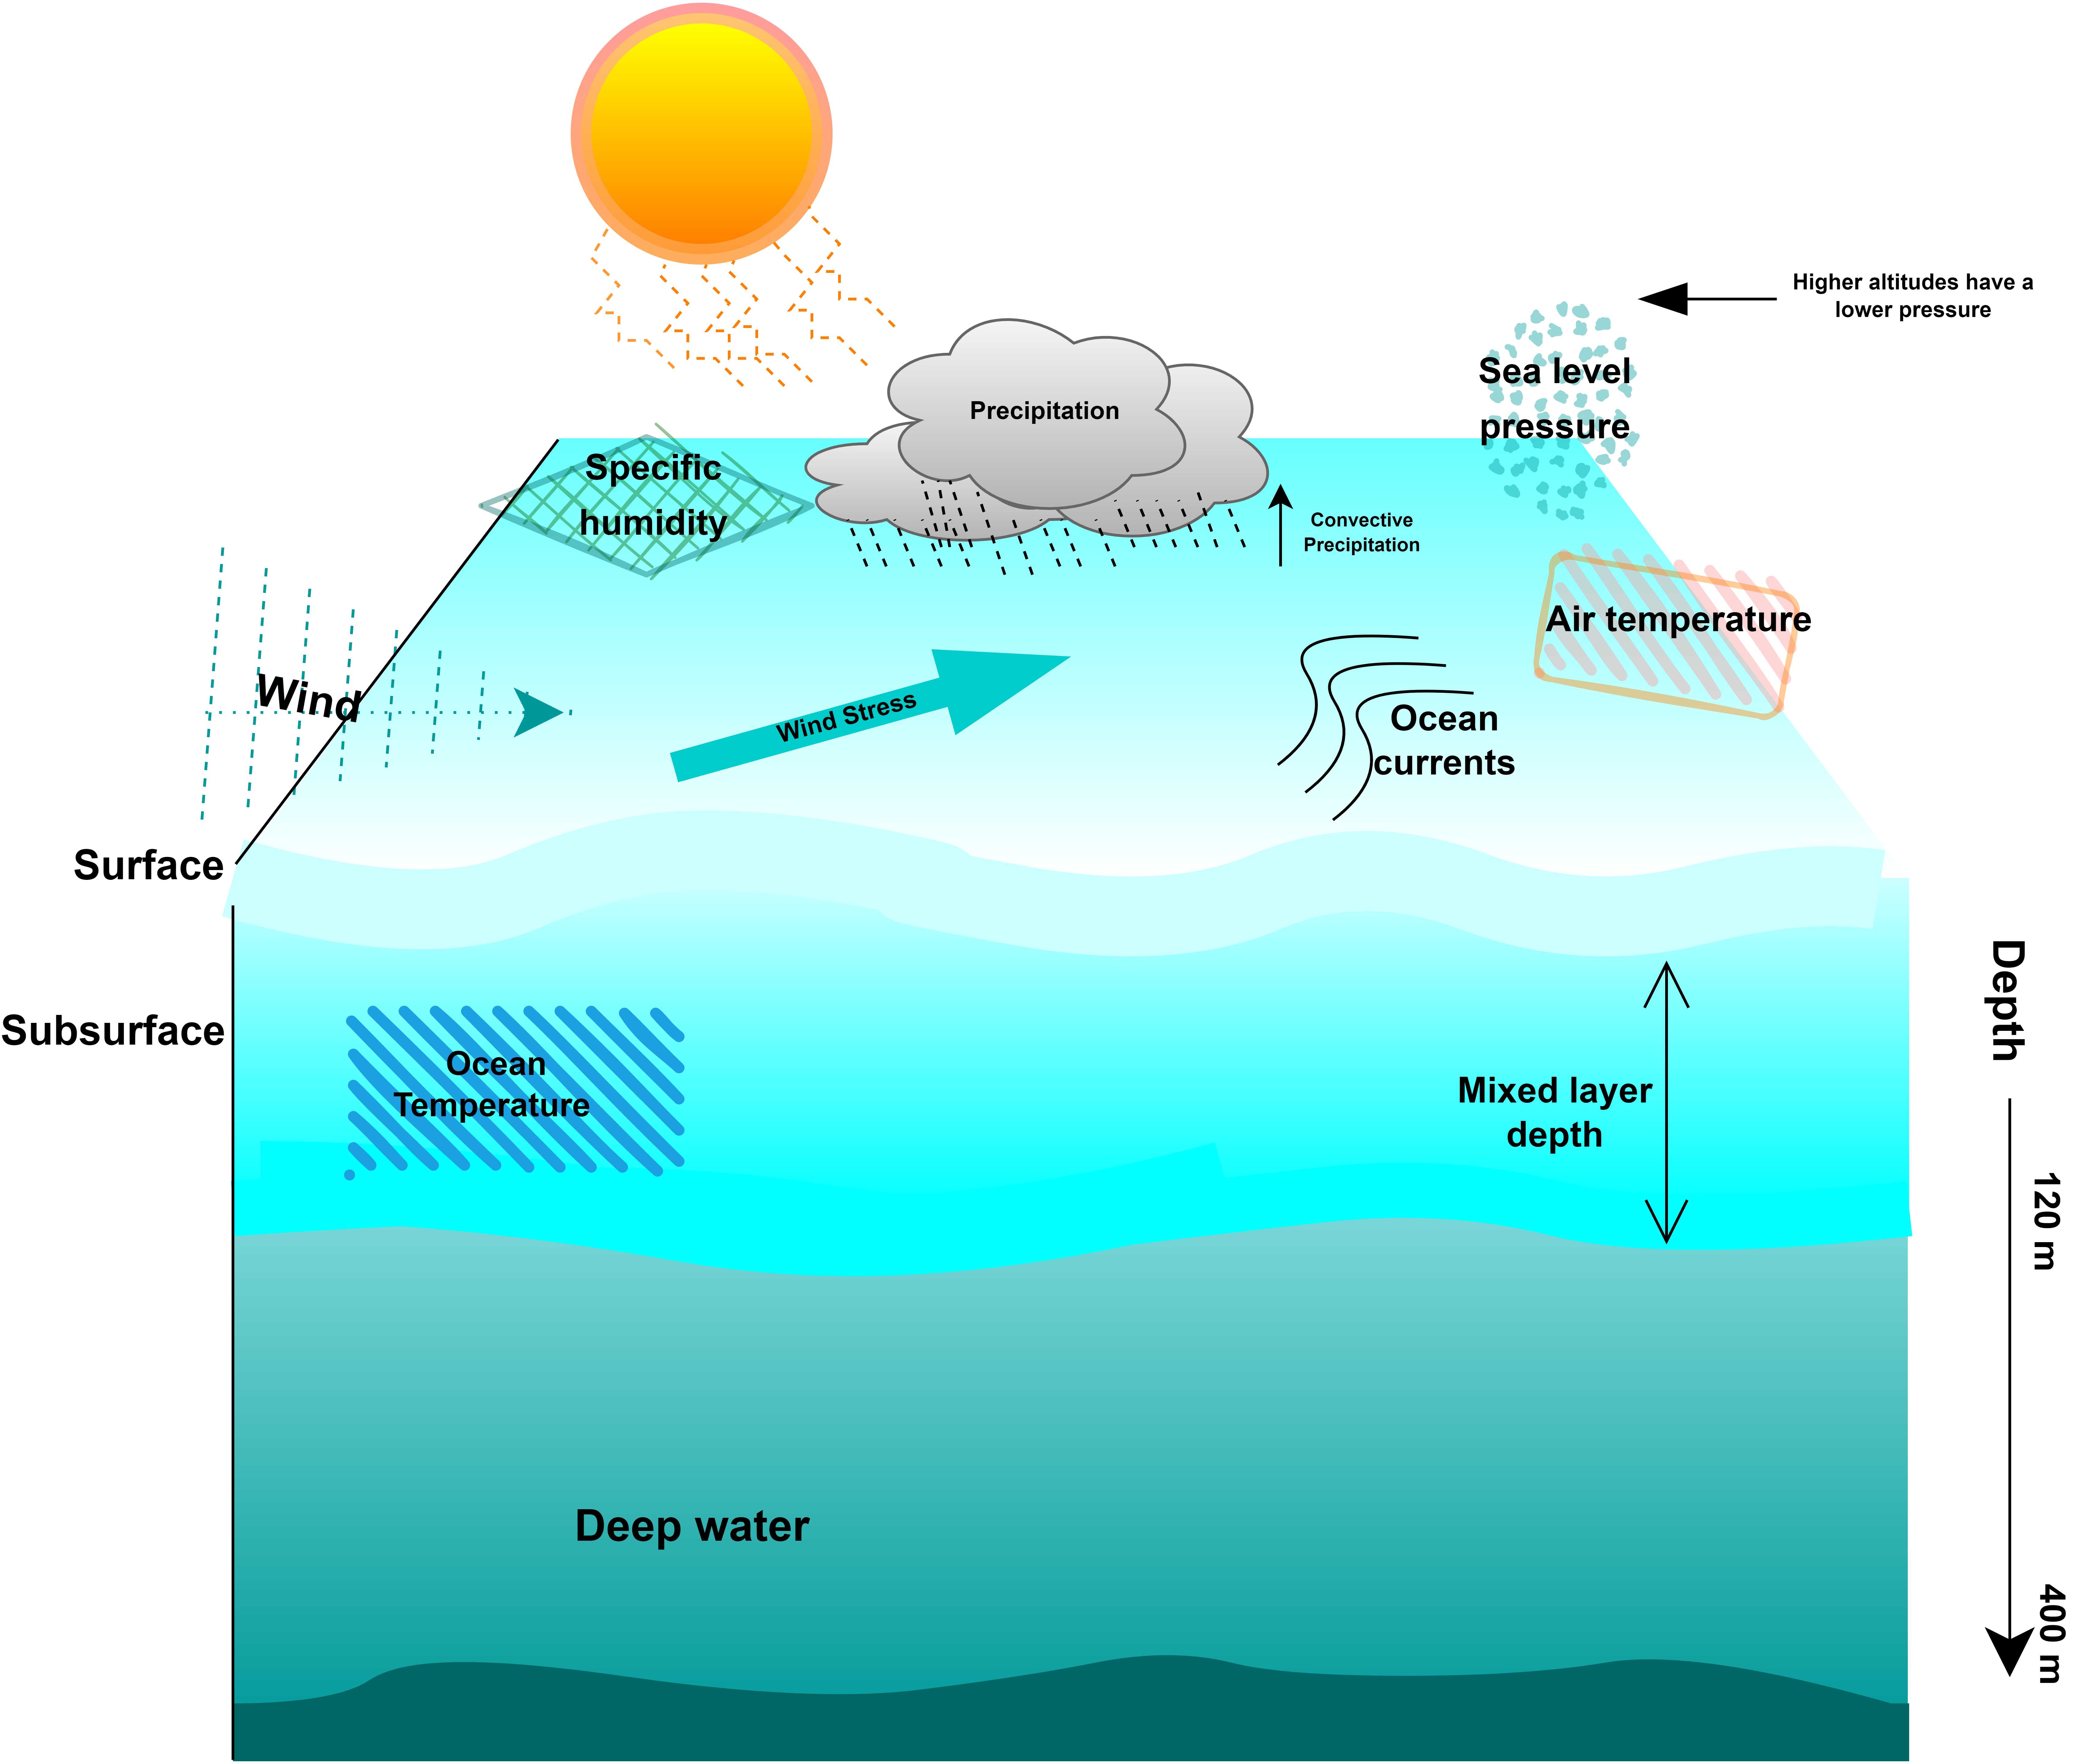
\includegraphics[width=15cm]{contents/MLD_Illustration}
		\caption{Diagram skematik yang menunjukkan interaksi yang terjadi pada antarmuka udara-laut yang melibatkan parameter-parameter meteorologi dan kedalaman lapisan campuran.}
		\label{fig:mld_illustration}
	\end{figure}
	$\textbf{\textit{Mixed layer depth} (MLD)}$ dapat ditentukan dengan menggunakan temperatur, salinitas, ataupun densitas. MLD yang berkaitan dengan temperatur dapat berupa temperatur yang cukup konstan pada kedalaman $100 - 200$m. \textit{Mixed layer} atau lapisan campuran adalah hasil dari pengaruh angin permukaan, gelombang, dan arus yang mencampur air bagian atas dan mendistribusikan panas ke seluruh lapisan ini. Di bawah lapisan campuran terdapat penurunan temperatur yang cepat sejalan dengan peningkatan kedalaman lautan. Lapisan ini disebut sebagai $\textbf{\textit{thermocline}}$. Di bawah lapisan termoklin, temperatur laut dalam cukup konstan sekitar $2^\circ$C yang terus turun hingga ke dasar laut. Ada sedikit perubahan temperatur di laut dalam, karena jauh dari sumber panas yang signifikan, menjadikannya salah satu daerah yang paling stabil secara termal di bumi.
	\begin{figure}[H]
		\centering
		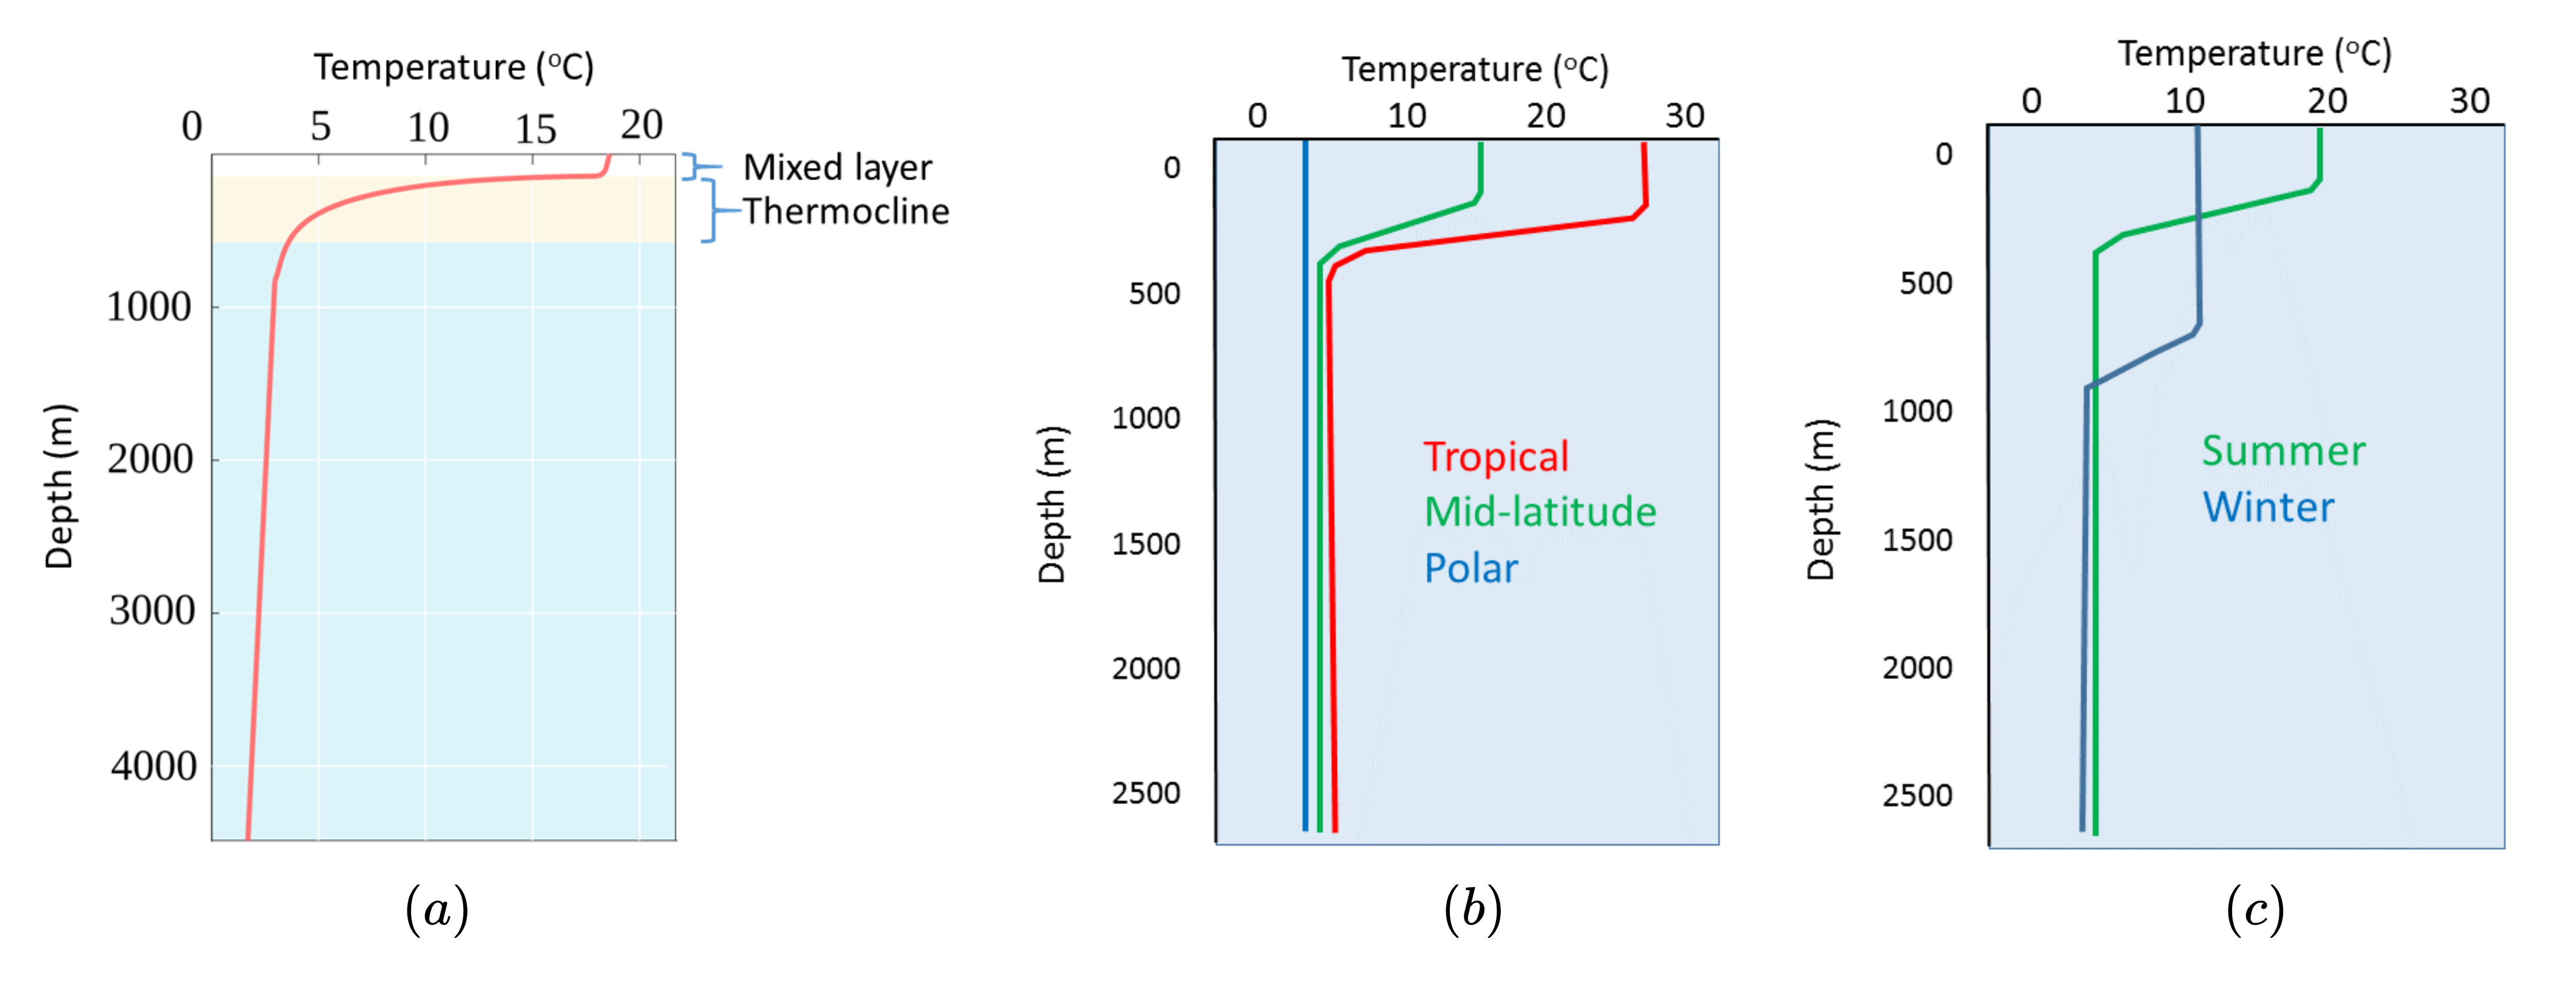
\includegraphics[width=15cm]{contents/mld_theory}
		\caption{(a) Profil temperatur laut terbuka yang khas untuk wilayah lintang tengah, menunjukkan lapisan campuran, termoklin yang curam, dan temperatur yang relatif stabil di kedalaman, (b) Profil temperatur representatif untuk daerah tropis, lintang tengah, dan kutub, dan (c) Di daerah beriklim sedang, lapisan campuran lebih dalam dan termoklin kurang menonjol di musim dingin dibandingkan dengan musim panas  \protect\shortcite{webb2021introduction}}
		\label{fig:mld_theory}
	\end{figure}
	 Profil temperatur bervariasi pada garis lintang yang berbeda, karena air permukaan lebih hangat di dekat khatulistiwa dan lebih dingin di kutub. Di daerah tropis lintang rendah, permukaan laut jauh lebih hangat, yang mengarah ke termoklin yang sangat menonjol (lihat Gambar \ref{fig:mld_theory}b). Selain itu, tidak banyak perubahan musiman pada temperatur permukaan di daerah tropis, sehingga hanya ada sedikit perubahan musiman di profil temperatur. Di daerah lintang tinggi (kutub), ada sedikit perbedaan antara temperatur permukaan dan temperatur air dalam, dan temperatur cukup konstan di semua  kedalaman. Oleh karena itu, perairan kutub tidak memiliki termoklin yang kuat, dan seperti halnya air tropis, hanya ada sedikit perubahan temperatur musiman. 
	 
	 Daerah beriklim sedang (lintang tengah) menunjukkan fluktuasi musiman yang lebih besar pada temperatur permukaan daripada kutub atau daerah tropis; perbedaan $8-15^\circ$C dari musim panas ke musim dingin di zona beriklim sedang, dibandingkan dengan hanya $\sim 2^\circ$C di daerah kutub dan tropis. Di daerah beriklim sedang, air permukaan jauh lebih hangat di musim panas dan termoklin lebih menonjol dibandingkan dengan musim dingin. Tetapi di musim dingin termoklin lebih dalam di garis lintang tengah daripada di musim panas. Ini karena badai musim dingin mengaduk-aduk air permukaan lebih banyak daripada yang terjadi di musim panas, menciptakan termoklin yang lebih dalam dan dengan demikian lebih dalam (lihat Gambar \ref{fig:mld_theory}c).
\end{spacing}
\vspace{-0.1pc}
%\section[Parameter Meteorologi]{Parameter Meteorologi}
%\begin{spacing}{1.5}
%
%\end{spacing}
